\section[Koincidenční metoda \& spektrometrie gama]{Koincidenční metoda stanovení aktivity a spektrometrie záření gama jako sekundární metoda měření aktivity}

\subsection{Koincidenční metoda}

Využívá se faktu, že při radioaktivní přeměně nuklidu dochází často k emisi vícero záření/částic. V praxi se jedná o využití dvou detektorů, kdy každý je citlivý na jiný druh záření a výstup, resp. impuls na výstupu čítače koincidencí je jen v případě, když dojde k "současnému" výskytu impulsů na obou detektorech (vstup A i B). Je nutné, aby impulsy byly zaznamenány v rámci tzv. rozlišovací doby. V opačném případě není zaznamenána koincidence, ale pouze výstup na čítači A či B.

\begin{figure}[H]
\centering
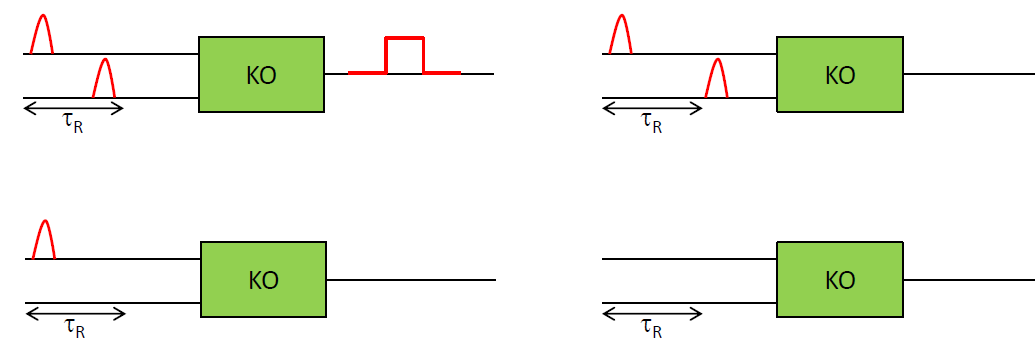
\includegraphics[width=0.7\linewidth]{img/koin-obvod.png}
\end{figure}

\begin{figure}[H]
    \centering
    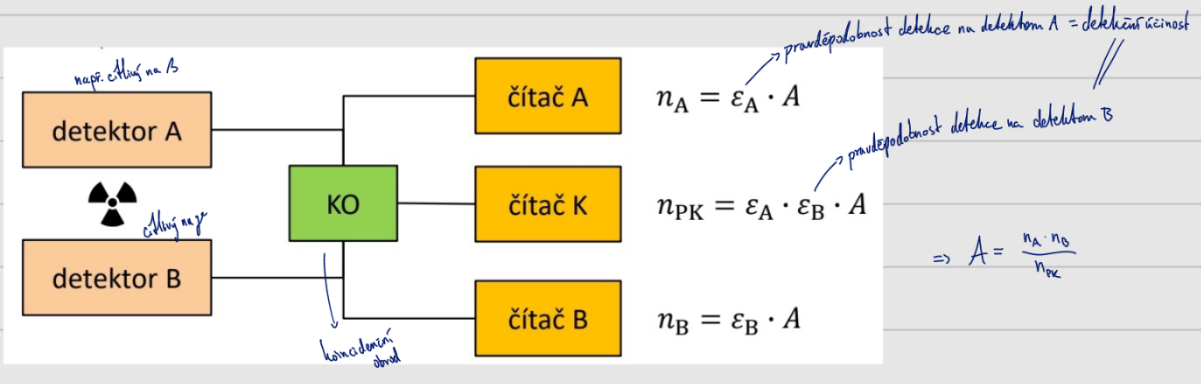
\includegraphics[width=\linewidth]{img/jednoduché koincidenční zapojení.png}
    \caption{jednoduché koincidenční zapojení}
\end{figure}

\textbf{Rozlišovací doba} může být stanovena dvěma způsoby, a to:

\begin{itemize}
    \item Generátor -- Pomocí generátoru si mohu nastavovat časový interval mezi generovanými signály a měřit jak citlivý je detekční systém na různé časové intervaly. Postupně se mění rozlišovací doba a sleduje se, kdy systém správně detekuje koincidenci.
    \item Náhodné koincidence -- Postupně se snižuje rozlišovací doba a měří se náhodné koincidence. Jakmile začne počet zaznamenáných koincidencí výrazně klesat, začiná se přibližovat optimální rozlišovací době. Cílem je najít takovou rozlišovací dobu, která minimalizuje počet náhodných koincidencí zatímco stále zachovává koincidence, které chci měřit.
\end{itemize}

Důležité je však znovu zdůraznit, že do celkového počtu koincidencí se mi projeví jak pravé tak náhodné koincidence a proto je žádoucí nastavit rozlišovací dobu správné.

\begin{figure}[H]
    \centering
    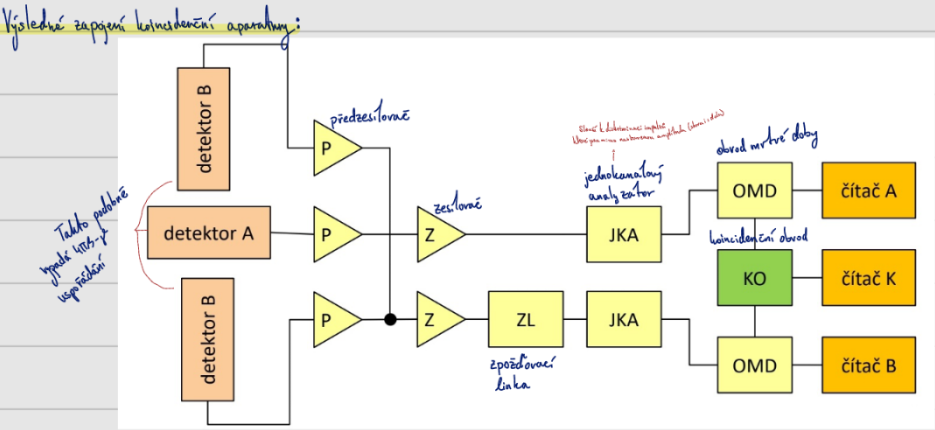
\includegraphics[width=1\linewidth]{img/Výsledné zapojení koincidenčního obvodu.png}
    \caption{Výsledné zapojení koincidenčního obvodu}
\end{figure}

Dobré vědět k čemu slouží jednotlivé komponenty:

\begin{itemize}
    \item \textbf{Detektor} = záznam/detekce signálu od IZ.
    \item \textbf{Předzesilovač} = Jeho hlavním úkolem je zesílit slabé signály z detektoru na úroveň, která je dostatečná pro další zpracování. Důležité je, aby zesílení proběhlo bez výrazného zvýšení šumu (změnou nastavení impedance), což by mohlo negativně ovlivnit kvalitu signálu. Další úlohou je přivedení pracovního napětí na detektor.
    \item \textbf{Zesilovač} = zvyšuje úroveň signálu, který již byl zesílen předzesilovačem, na úroveň vhodnou pro zpracování dalšími elektronickými obvody, jako je například jednokanálový analyzátor. Musí poskytnout stabilní a lineární zesílení signálu, aby nedocházelo k deformaci (zkreslení) původního signálu
    \item \textbf{Zpožďovací linka} = záměrně zpožďuje signál přicházející z detektoru o určitou dobu. Její hlavní funkcí v koincidenčním měření je zajistit, aby signály z různých detektorů dorazily do koincidenčního obvodu ve správném časovém rozmezí, i když mají různé dráhy nebo rychlosti zpracování. To je důležité pro správnou identifikaci koincidenčních událostí, protože signály musí dorazit téměř současně, aby byly považovány za koincidentní.
    \item \textbf{JKA} = Jednokanálový analyzátor slouží k selekci signálů podle jejich amplitudy, což odpovídá energii detekovaného záření. Signál má tak posléze formu 1 nebo 0, tedy splňuje nebo nesplňuje. Propustí pouze ty signály, jejichž amplituda spadá do definovaného rozsahu (dolní hranice stanovená diskriminací).
    \item \textbf{Obvod mrtvé doby} = Obvod mrtvé doby je navržen tak, aby po detekci jednoho signálu zablokoval možnost detekce dalších signálů po určitou dobu. Mrtvá doba je důležitá pro zabránění registrace falešných koincidenčních událostí způsobených příliš blízkými nebo souběžnými událostmi, které by mohly být mylně považovány za koincidentní.
    \item \textbf{Koincidenční obvod}
    \item \textbf{Čítač}
\end{itemize}

\subsubsection{Instrumentální opravy}

\begin{itemize}
    \item Korekce na pozadí, náhodné koincidence a mrtvou dobu.
    \item Aplikace koincidenční metody: 
    \item 
    \begin{itemize}
        \item 4$\pi \, \beta - \gamma$: nuklidy $^{24}$Na, $^{42}$K, $^{56}$Co, $^{59}$Fe $\rightarrow$ při této koincidenční metodě je RN vložen do interního počítače (měření $\beta$) a okolo počítače jsou např. scintilační detektory pro měření $\gamma$. Celé je to posléze stíněné pro minimalizaci vlivu pozadí.
        \item 4$\pi \, \alpha - \gamma$: $^{210}$Po, $^{241}$Am
    \end{itemize}
\end{itemize}

\subsubsection{Korekce -- Opravy jednoduchého jaderného schématu}

\begin{itemize}
    \item Vnitřní konverze -- vyzáření elektronu z obalu (konverzní elektron) a u toho vzniká ještě doprovodné charakteristické RTG záření => detekce KE v $\beta $ kanálu. Není to to samé jako Beta přeměna. Jedná se o konkurenční proces k emisi fotonu při deexcitaci. Oprava probíhá úpravou vztahu pro výpočet elektronů v $\beta$ kanálu, tedy poměr naměřených četností/aktivita. 
    \item Citlivost kanálu $\beta$ na záření $\gamma$ řeším úpravou koincidenční rovnice. V opačném případě, kdy jsou elektrony v $\gamma$ kanálu, lze využít například stínění detektorů, kterým částice Beta neprojde.
    \item Brzdné záření -- většinou zanedbatelně malý vliv, ale dělá to vliv záření $\beta$ na detektor citlivý na $\gamma$. Pokud chceme, tak se opět mohou dělat opravy koincidenční rovnice. Možná by se toho šlo zbavit vhodným nastavením diskriminace?
\end{itemize}

\subsubsection{Metody}

\begin{itemize}
    \item \textbf{Extrapolační metoda} -- Spočívá v uskutečnění série měření pro různé hodnoty detekční účinnosti v kanále $\beta$ ($\varepsilon_\beta = \frac{n_k}{n_\gamma}$), čehož docílíme např. překrytím vzorku filmem či změnou diskriminace/zesílením (upravuji účinnost v kanále $\beta$). Výsledná závislost (účinnost na $\frac{n_\beta \cdot n_\gamma}{n_{PK}}$ ) (viz rovnice níže) je lineárně proložena a extrapolována k nule (s -> 0). Všechny výše zmíněné opravy lze uvažovat ve společném tvaru 
    
    $$M = \dfrac{n_{\beta} n_{\gamma}}{n_{PK}} = A \cdot [1 + S\cdot k] $$

    \item \textbf{Stopovací metoda} -- Přimíchám čistý ZIZ $\beta$ se vzorkem $\beta-\gamma$, použiju přincip extrapolační metody (získám měření pro různé poměry aktivity vzorku a celku). V praxi funguje tak, že smíchám čistý zdroj IZ $\beta$ a vhodný radionuklid s kaskádou $\beta - \gamma$. Posléze měřím celkovou aktivitu směsi ($A_{xs}$) a aktivitu RN s kaskádou ($A_s$). Odečtením jednoho od druhého dostanu aktivitu čistého zdroje IZ $\beta$ ($A_x$) => $A_{xs} = A_x + A_s$.
    
    \item záchytové radionuklidy -- měřím koincidenci záření X$_{\text{K}}$ a X$_{\text{L}}$ - čistý záchyt elektronu
    \item záchytové radionuklidy -- měřím koincidenci záření X - $\gamma$ - obdoba kaskádám $\alpha - \gamma$, větší uplatnění korekčních faktorů, oboje měření se záchytovými radionuklidy je těžší na provedení, neboť si zde konkurují různé proces
\end{itemize}

\subsection{Spektrometrie gama jako sekundární metoda měření aktivity}

\textbf{Interakce fotonů s látkou:}

\begin{itemize}
    \item Fotoelektrický jev (energie fotonů je zpravidla nejmenší) -- energie je všechna předána elektronu a dochází k jeho vyražení z elektronového obalu. Jeho prázdné místo je zabráno elektronem z vyšší energetické hladiny/slupky a rozdíl energií je vyzářen v podobě RTG charakteristického záření.

    \item Comptonův rozptyl: (vyšší energie gama fotonů) -- část energie je předána elektronů a dochází k jeho vyražení. Platí, že fotoefekt je závislý na hmotnostním čísle, ale Comptonův jev není, a proto je pro lehká jádra pravděpodobnější Comptonův rozptyl.

    \item Tvorba elektron-positronového páru -- energie iniciujícího fotonu musí být vyšší než je 1,02 MeV (2x511 keV) a ideálně o něco vyšší. Dochází k přeměně fotonu v blízkosti jádra atomu na pár elektron a positron. Přebytek energie je předán jádru v podobě hybnosti. Při jejich zániku rekombinací vzniká tzv. anihilační fotony, které mají 2x$\gamma$ pod úhlem 180$^\circ$ o velikosti 2x511 keV. Tato energie je tam dána jako podmínka, protože klidová energie, resp. hmotnost elektronu i positronu je 511 keV.
\end{itemize}

\begin{figure}[H]
\centering
	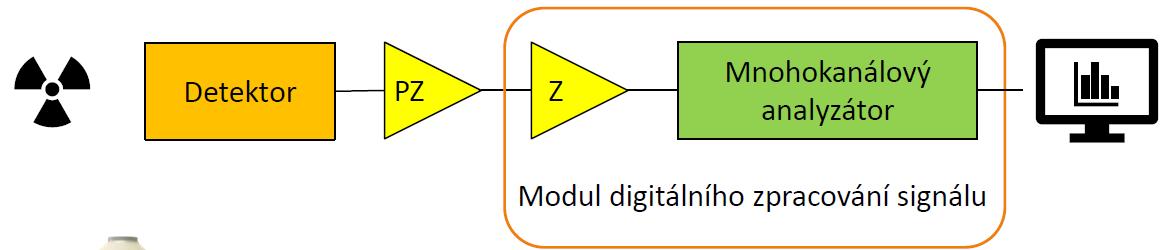
\includegraphics[width=0.8\linewidth]{img/spek-trasa.png}
	\caption{Spektrometrická trasa}
\end{figure}

MCA = Mnohokanálový analyzátor -- počítá impulzy z detektoru v závislosti na velikosti jejich amplitudy. Umožňuje nastavovat počet kanálů (jejich šířka energií), diskriminace, oprava na mrtvou dobu, zesílení, ...

\textbf{Detektory pro spektrometrii gamma}: jedná se o materiály s vysokým protonovým číslem.

\begin{itemize}
    \item Scintilační detektory = NaI(Tl), LaBr$_3$(Ce), CsI(Tl) => Mají vyšší účinnost a nemusí být chlazeny (možný provoz za pokojové teploty).
    \item Polovodičové detektory = Vysoké energetické rozlišení, ale nutno při provozu chladit na teplotu kapalného dusíku. (HPGe, Si(Li)).
    \item Je dobré mít zajištěné vhodné stínění, na čež se používají materiály s vysokým hmotnostním číslem a také vícevrstvé řešení (Pb, Cd, Cu).
\end{itemize}


\textbf{Spektrum detektorů různých velikostí:}

\begin{itemize}
    \item Malé detektory = rozměr je menší než střední volná dráha rozptýleného fotonového záření. Spektrum je tak tvořeno Comptonovým kontinuem, DEP a píkem úplné absorpce.

\begin{figure}[H]
    \centering
    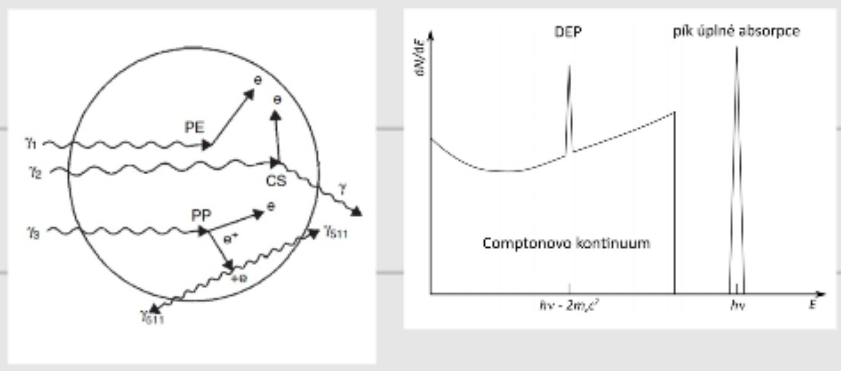
\includegraphics[width=0.75\linewidth]{img/male detektory spektrum.png}
    \caption{male detektory spektrum}
\end{figure}
    
    \item Středně velké detekotry = rozměr je srovnatelný se střední volnou dráhou, a proto spektrum obsahuje to samé co pro malé detektory, ale dále navíc SEP a část spektra náležící vícenásobnému rozptylu.

\begin{figure}[H]
    \centering
    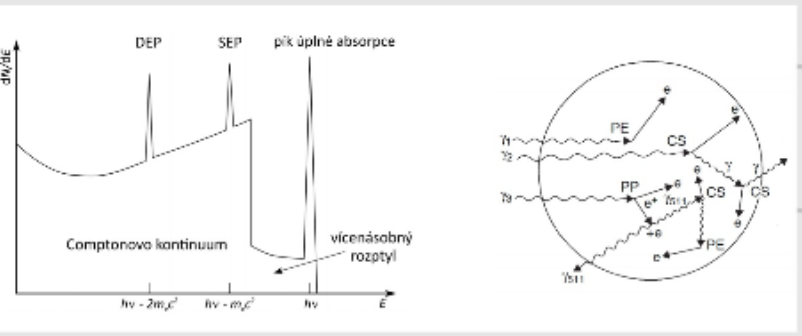
\includegraphics[width=0.75\linewidth]{img/Středně velké detekotry spektrum.png}
    \caption{Středně velké detekotry spektrum}
\end{figure}
    
    \item Velké detektory = Všechny události přispívají do píku úplné absorpce.

\begin{figure}[H]
    \centering
    \includegraphics[width=0.75\linewidth]{img/Velké detektory spektrum.png}
    \caption{Velké detektory spektrum}
\end{figure}
    
\end{itemize}

\textbf{Spektrometrické stanovení aktivity:}

Stanovení aktivity na základě plochy píku, píkové účinnosti, radiačního výtěžku a živé doby měření. 

Deteční účinnost se pak ještě dělí na absolutní, vnitřní, celkovou a píkovou, kde detekční účinnost obecně znamená podíl počtu částic, které jsou zaznamenány a počet částic emitovaných zdrojem. Píková detekční účinnost obsahuje pouze interakce, jenž patří do píku úplné absorpce.

\begin{equation}
    A = \frac{P}{\varepsilon Y t}
\end{equation}